% Math symbols and examples: http://en.wikibooks.org/wiki/LaTeX/Mathematics
% Also useful link: http://en.wikibooks.org/wiki/LaTeX/Advanced_Mathematics

% This document is used for title generating of exercise solutions. 
% Also it used for generating styles and environmentof documents.
% To add this title in document add next line:
% % This document is used for title generating of exercise solutions. 
% Also it used for generating styles and environmentof documents.
% To add this title in document add next line:
% % This document is used for title generating of exercise solutions. 
% Also it used for generating styles and environmentof documents.
% To add this title in document add next line:
% \input{../template.tex}
\documentclass[a4paper]{article}
\usepackage[utf8]{inputenc}
\usepackage[top=1.5cm]{geometry}
\usepackage{amssymb}
\usepackage{enumitem}
\usepackage{amsmath}

\allowdisplaybreaks

\DeclareMathOperator{\ggT}{ggT}
\DeclareMathOperator{\kgV}{kgV}

\title{Mathematik: Diskrete Strukturen \\ \Large Lösungsblatt}
\author{Anton Bubnov, Eugen Kuzmenko}

\documentclass[a4paper]{article}
\usepackage[utf8]{inputenc}
\usepackage[top=1.5cm]{geometry}
\usepackage{amssymb}
\usepackage{enumitem}
\usepackage{amsmath}

\allowdisplaybreaks

\DeclareMathOperator{\ggT}{ggT}
\DeclareMathOperator{\kgV}{kgV}

\title{Mathematik: Diskrete Strukturen \\ \Large Lösungsblatt}
\author{Anton Bubnov, Eugen Kuzmenko}

\documentclass[a4paper]{article}
\usepackage[utf8]{inputenc}
\usepackage[top=1.5cm]{geometry}
\usepackage{amssymb}
\usepackage{enumitem}
\usepackage{amsmath}

\allowdisplaybreaks

\DeclareMathOperator{\ggT}{ggT}
\DeclareMathOperator{\kgV}{kgV}

\title{Mathematik: Diskrete Strukturen \\ \Large Lösungsblatt}
\author{Anton Bubnov, Eugen Kuzmenko}

\usepackage{ tipa }
\usepackage{tikz}

\begin{document}
    \maketitle
    \section*{Vertiefung:}
    \begin{enumerate}[label=(\alph*)]
        % Task (a)
        \item Bestimmen Sie $\chi(Q_3)$.\\
        Nach Vertiefung (j) (Blatt 9) $\chi (Q_3) = 2$. 
                
        % Task (b)
        \item Bestimmen Sie $\chi(Q_4)$.\\
        Nach Vertiefung (j) (Blatt 9) $\chi (Q_4) = 2$.        
                
        % Task (c)
        \item
               
        % Task (d)
        \item Bestimmen Sie $\chi'(Q_3)$.\\
        Nach Vizing folgt: $\chi'(Q_3) = 3$ (Theorem 3.31).
        
        %Task (e)
        \item
        
        %Task (f)
        \item Gilt $\chi ' (G) = k $ für jeden k-regulären Graphen G? \\
        Nein. Man betrachte hierzu den $K_3$. Dieser Graph ist vollständig aber 2-regulär (k=2), da jeder Knoten mit 2 Knoten in Verbindung steht. Somit folgt hieraus mit $\chi'(K_3) = 3 \neq 2$ ein Widerspruch.
        
        %Task (g)
        \item 
        Angenommen es gibt zwei perfekte Matchings in einem Baum. Dann müsste für jeden Knoten $v \in V$ folgendes gelten: $\textrm{deg}(v) = 2$, da beide Matchings unterschiedlich sein müssen und jeder Knoten an jeweils einer Kante aus dem einen Matching und aus einer Kante vom anderen Matching beteiligt sein muss. Dann haben wir allerdings einen Widerspruch zur Definition des Baumes, denn ein Knotengrad von 2 bei allen Knoten des Graphen impliziert, dass der Graph einen Kreis enthalten muss (bzw. selbst einer ist). Somit kann ein Baum nicht mehr als ein perfektes Matching enthalten. 
        
        %Task (h)
        \item 
        Welche Gitter $M_{n,m} $enthalten perfekte Matchings? \\
        Der $M_{n,m}$ hat $n \cdot m$ Knoten. Wenn $n$ und $m$ beide ungerade sind, dann besteht der $M_{n,m}$ ebenfalls aus einer ungeraden Anzahl aus Knoten. Nach der Definition 3.32 (2.) muss $||M|| = \frac{1}{2} ||V||$ gelten, damit ein perfektes Matching gefunden werden kann. Wir können demnach kein perfektes Matching finden, da es keinen Graphen mit ''halben Knoten'' geben kann. \par
        Für den Fall das $n \cdot m$ gerade ist, lässt sich ein perfektes Matching für einen $M_{n,m}$ darstellen, indem man die Knoten links außen vom Gitter nimmt und ''paarweise nach rechts Verknüpft'', wobei bereits gematchte Knoten überspruchgen werden müssen. Folgende Graphik veranschaulicht den Gedanken:
        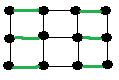
\includegraphics{task_h}[h]
        Folglich hat der $M_{n,m}$ ein perfektes Matching, für den Fall, dass $n \cdot m$ gerade ist.
        
        %Task (i)
        \item
        Wieviele perfekte Matchings enthält der $Q_3$? \\
        9
        %Task (j)
        \item 
        Wieviele perfekte Matchings enthält der $K_{2n}$ ?
        
    \end{enumerate}
    \section*{Kreativität:}
    \begin{enumerate}[label=(\alph*)]
    	%Task (a)
    	\item Task a
    \end{enumerate}
    \section*{Transfer:}
    \begin{enumerate}[label=(\alph*)]
    	\item Bestimmen Sie das kleinste r, sodass G r ein perfektes Matching enthält.\\
        Überschreiben wir gegebene Tabellen in eine. Da wir können deutlich sehen, dass kleinste $r=4$. %5 oder?
        \begin{table}
            \begin{tabular}{|l|c|c|c|c|c|c|}
            \hline
            ~          & Hause     & Whipcat   & Adobra    & Dottie    & Badhitee  & Culture   \\ \hline
            Biscuit    & {\bf 1,1} & 2,1       & 6,1       & 4,1       & 5,1       & 3,1       \\ \hline
            Adagio     & 1,2       & 3,4       & {\bf 4,3} & 2,5       & 5,2       & 6,6       \\ \hline
            Sobresalto & 3,3       & 4,2       & 2,6       & 5,3       & 6,4       & {\bf 1,2} \\ \hline
            Apera      & 4,4       & {\bf 2,3} & 6,4       & 3,4       & 1,5       & 5,3       \\ \hline
            Cyrano     & 2,5       & 1,5       & 4,5       & 5,6       & 3,6       & 6,4       \\ \hline
            Happy      & 1,6       & 3,6       & 5,2       & {\bf 2,2} & {\bf 4,3} & 6,5       \\ \hline
            \end{tabular}
        \end{table}
        \item Bestimmen Sie ein perfektes Matching, sodass es keine unzufriedenen Paare gibt.\\
        Verwenden wir dafür Gale - Shapley Algorithm. Dann bekommen wir:
        \begin{table}
            \begin{tabular}{|l|c|c|c|c|c|c|}
            \hline
            ~          & Hause     & Whipcat   & Adobra   & Dottie   & Badhitee   & Culture   \\ \hline
            Biscuit    & {\bf 1,1} & 2,1       & 6,1      & 4,1      & 5,1        & 3,1       \\ \hline
            Adagio     & 1,2       & {\bf3,4}  & 4,3      & 2,5      & 5,2        & 6,6       \\ \hline
            Sobresalto & 3,3       & 4,2       & 2,6      & 5,3      & 6,4        & {\bf1,2}  \\ \hline
            Apera      & 4,4       & 2,3       & 6,4      & 3,4      & 1,5        & 5,3       \\ \hline
            Cyrano     & 2,5       & 1,5       & {\bf4,5} & 5,6      & 3,6        & 6,4       \\ \hline
            Happy      & 1,6       & 3,6       & 5,2      & {\bf2,2} & {\bf4,3}   & 6,5       \\ \hline
            \end{tabular}
        \end{table}
    \end{enumerate}
\end{document}






